A Master’s thesis in engineering usually consists of an
implementation part (literature survey, hardware development,
software development, measurements, etc.), and a written part (the
text body). How the implementation part is carried out depends on the
topic, so no general guidelines can be issued. However, each type of
publication has its distinct layout and structure to be followed. The
following set of instructions will explain in detail the writing and
layout style for the master’s theses published in the engineering
degree programmes at the Faculty of ITEE. Typography affects the
readability of the text greatly, so the instructions should be
followed strictly. By following these instructions, the thesis
authors can properly learn a proper way of expressing themselves
formally in writing. After having learned one way of formal writing,
it is easier to get used to the formalism used at your future
workplace. Presentation and layout style have an effect on the grade
of the thesis.

Before starting to write your thesis, it is a good idea to mind-map
or chart out the various issues that will be included in a thesis.
After that, you should divide them into themes, actual chapters with
actual title, and estimated numbers of pages to be included in each
chapter. The contents should be discussed in detail with your
principal supervisor. Pay attention on the weighting and focus of
different topics. You should reserve enough time for writing your
thesis, so that its content and structure will be as good as
possible. It should be remembered that the archived thesis book is
usually the only document through which your whole thesis work will
later be assessed.

\section{Linguistic style}
\label{sec:linguistic_style}

As a general rule, students who have completed their matriculation
exam in Finland write their Master’s thesis in Finnish or Swedish.
Foreign students who are not fluent in Finnish write their thesis in
English. The thesis can be also written in English if it is
well-justified, for example, when the supervisor or the project team
does not understand Finnish well enough.

The language of a thesis written in English has to be flawless. If
the thesis does not meet this requirement, or the principal
supervisor feels that she/he is not capable of checking the language
well enough, the supervisor can demand the thesis to be checked by a
proofreading company, a person qualified to edit technological
vocabulary in English, a native English speaker, or a person holding
the degree of M.A. in English Philology. One should notice that the
correctness of the language affect the grading of the thesis.

The thesis should have an abstract and a title in both English and
Finnish. The only exceptions are the international master’s degree
students who do not need to have the Finnish abstract or title. If
the language of the thesis is English, the abstract in English comes
before the abstract (tiivistelmä) in Finnish.

A Master’s thesis is written for an engineering audience. The author
should therefore avoid presenting issues and topics that go beyond
this scope. You should apply professional terminology when available.
This rule also applies to all figures and tables.

The aim is a clear and well-structured thesis, \textbf{without
unnecessary excessive use of words}---a thesis usually has 50--80
pages. The language (English/Finnish/ Swedish) should be fluent and
readable, and it should adhere to the conventions and recommendations
applied in a particular language. Advice on such issues can be
obtained from various language guides (in Finnish,
e.g.,~\cite{maamies}). There are also several excellent sources on
the internet, e.g.,~\cite{korpela, kielitoimisto} in Finnish
and~\cite{reportwriting, englishlanguage} in English.

\section{Typography}

In the text typography, you need to use the following guidelines and rules:

\begin{itemize}
    \setlength\itemsep{0pt}
    \setlength\parskip{0pt}
  \item Font: Times New Roman
  \item Page margin settings (exception: physical, bound copies use different settings; see Section~\ref{boundversion}):
    \begin{itemize}[wide=0pt]
        \setlength\itemsep{0pt}
        \setlength\parskip{0pt}
      \item Left margin: 2,5 cm
      \item Right margin: 2,5 cm
      \item Top margin: 2,5 cm
      \item Bottom margin: 3,0 cm
    \end{itemize}
  \item Spacing:
    \begin{itemize}[wide=0pt]
        \setlength\itemsep{0pt}
        \setlength\parskip{0pt}
      \item Before a heading: 2 empty rows
      \item After a heading: 1 empty row
      \item Between two headings: 1 empty row
      \item Line spacing: the default value for each font size, which
        is usually the font size 2 pts.
      \item The space between two paragraphs is a normal line spacing
      \item There is no indent in the first paragraph following a
        heading, but the following
        paragraphs are indented by 0.5 cm
      \item A single empty line is added between table and figure
        captions and the basic text
    \end{itemize}
\end{itemize}

\subsection{Figures and tables}
The thesis should include figures and tables to support the text.
They should be placed in the following manner as is automatically
done when following the model of this \LaTeX\ template:

\begin{itemize}
    \setlength\itemsep{0pt}
    \setlength\parskip{0pt}
  \item Table structure and the different fonts used in different
    instances are explained in \tabref{tab:sample_table}.
  \item In tables, the heading has to be placed above the table. The
    table heading should not end in a full stop. The permission to
    publish a table copied from another source has to be mentioned as
    part of the table heading. Many publishers inform the correct
    form to write this permission when such a permission has been
    granted. The table must be in text format – not an image.
  \item If necessary, the caption should be separated from the figure
    with a single line spacing for reasons of clarity. A figure and a
    short caption are centered. However, a caption spanning multiple
    lines is justified at both ends. The necessary references are
    included in the figure captions. Copyright information is also
    added to the end of the caption. The permission to publish a
    figure copied form another source has to be mentioned as part of
    the figure text. Many publishers inform the correct form to write
    this permission when such a permission has been granted.  The
    copyright issues and citation practices of images are further
    discussed in~\secref{copyright}.
  \item Do not start a chapter with a figure, but embed it in the
    text content. A figure is supposed to always appear in the text
    after its reference. If there is not enough space for the figure
    directly after the first reference, the word processor moves the
    figure automatically to the next page. In such case, the figure
    can be moved forward so that text originally after the figure
    fills the empty space. However, a figure should always be placed
    in the same chapter---hence sometimes empty space at the bottom
    of some chapters cannot be avoided (the same rules applies for the tables).
\end{itemize}

\begin{table}[!ht]
  % Add some padding to the table cells:
  \def\arraystretch{1.1}%
  \begin{center}
    \caption{The font types used in a Master’s thesis}
    \label{tab:sample_table}
    \begin{tabular}{| c | l | l | l | l |}
      \hline
      \multicolumn{1}{|l|}{Font}  & \multicolumn{4}{l|}{Layout}
      \\\cline{2-5} \multicolumn{1}{|l|}{size} & Regular &
      \textbf{Bold} & \textit{Italic} & \textbf{\textit{Bold}} \\(pt)
      &  &  &  & \textbf{\textit{Italic}}\\
      \hline
      10 &  {\fontsize{10}{12pt}\selectfont Table and figure} &  &  &  \\
      &  {\fontsize{10}{12pt}\selectfont contents, footnotes,} &  &  &  \\
      &  {\fontsize{10}{12pt}\selectfont and endnotes} &  &  &  \\
      \hline
      12 & Standard text &  \textbf{1\textsuperscript{st} level} &
      \textit{3\textsuperscript{rd} level} &
      \textbf{\textit{2\textsuperscript{nd} level}}\\
      &  equations, &  \textbf{subheadings,} &  \textit{subheadings}
      &  \textbf{\textit{sub-}} \\
      & references, tables, & \textbf{abstract, abstract} &  &
      \textbf{\textit{headings}} \\
      & captions, table & \textbf{in Finnish} &  &  \\
      & headings & \textbf{(tiivistelmä)} &  &  \\
      \hline
      \rule{0pt}{0.8\normalbaselineskip}
      14 &  & {\fontsize{14}{17pt}\selectfont \textbf{CHAPTER}} &  &  \\
      &  & {\fontsize{14}{17pt}\selectfont
      \textbf{TITLE\textsuperscript{1}}} &  &  \\
      \hline
      \rule{0pt}{1.0\normalbaselineskip}
      16 &  & {\fontsize{16}{19pt}\selectfont \textbf{Author}} &  &  \\
      &  & {\fontsize{16}{19pt}\selectfont \textbf{name}} &  &  \\
      \hline
      \rule{0pt}{1.1\normalbaselineskip}
      {\fontsize{16}{19pt}\selectfont 18} &  &
      {\fontsize{18}{22pt}\selectfont \textbf{THESIS}} &  &  \\
      &  & {\fontsize{18}{22pt}\selectfont \textbf{TITLE}} &  &  \\
      \hline
    \end{tabular}
    \vspace{6pt}

  \raggedright \ \space \textsuperscript{1} Each full chapter should
  start on a new page.
\end{center}
\end{table}

You should not use single subsections---for example, Section 2.1
needs to be accompanied by Section 2.2. Also, please do not number
sections beyond the 3\textsuperscript{rd}  grade (e.g., 1.2.1.1
should not be used). Should the need arise for further decimalization
the following method below (a \textbf{bolded}, unnumbered heading
that does not appear in the table of contents) should be applied:

\subsubsection{Formatting the figure captions}
Figures, tables and appendices are a part of the written
presentation. All these need to be referenced to in the text body,
preferably before the figure is placed in the text---i.e., first the
referring text, then the figure or table. Figures and tables have a
running number through the document---or chapter wise, if there are
plenty of figures. \figref{fig:work_packages} serves as an example of a figure and a
text referring to it. Figure captions are below the figure, and the
caption text ends with a full stop. A short caption is centered,
while a long caption extending to a several lines is justified on both sides.

% Pictures in .pdf, .png or .jpg. No need to specify the extension.
% Transparent images are not allowed with PDF/A.
% With ImageMagick transparency can be removed with
% convert image.png -background white -alpha remove -alpha off image_nobg.png
% This restriction also affects PDF images, as a first step try to make the PDF
% image PDF/A:
% gs -dPDFA -dBATCH -dNOPAUSE
% -sColorConversionStrategy=UseDeviceIndependentColor
% -sDEVICE=pdfwrite -dPDFACompatibilityPolicy=2
% -sOutputFile=output.pdf input.pdf
\begin{figure}[ht]
\begin{center}
  \includegraphics*[width=0.7\textwidth]{WP}
\end{center}
\caption{Connections between work packages (WP).
  \copyrightstring\ \href{https://creativecommons.org/licenses/by/4.0/}{CC
BY 4.0}.}
\alt{Diagram showing interactions between work packages WP1 to WP5,
  all inside WP6, which is itself inside WP7. WP3 (left) sends
  outputs to WP1, WP2, and WP4. WP1 and WP2 are bidirectionally
  linked. WP1, WP2, and WP4 send outputs to WP5 (right). A curved
arrow shows WP3 also directly feeding into WP5.}
\label{fig:work_packages}
\end{figure}

If no external source is mentioned in the caption, it is assumed that
the thesis author is also the creator and copyright holder of the
figure (noting that authorship and copyright ownership are not always
the same). In such cases, the figure is licensed under the same terms
as the document itself (default: “All rights reserved”). This is
further discussed in \secref{copyright}. For figures that constitute
significant contributions — and may therefore be of interest for
reuse — it is advisable to explicitly state the copyright and
licensing information, even if it has already been included on a separate
copyright page.

Figures and tables should be given an alternative text that summarises
the information they contain for the reader. This is discussed further
in~\secref{accessibility}. Unfortunately support for this in
\LaTeX\ is still work in progress, and the alternative text will
currently not end up in the final PDF, so including them is not a requirement.
A suitable alternative text for~\figref{fig:work_packages} could be:

\begin{quote}
Diagram showing interactions between work packages WP1 to WP5, all
inside WP6, which is itself inside WP7. WP3 (left) sends outputs to
WP1, WP2, and WP4. WP1 and WP2 are bidirectionally linked. WP1,
WP2, and WP4 send outputs to WP5 (right). A curved arrow shows WP3
also directly feeding into WP5.
\end{quote}

The final thesis will be published as a PDF/A file, and this LaTeX
template produces files in that format directly. Be sure to remove all
transparency in your source images to ensure the end result is also
compliant. This affects figures in PDF and PNG formats. Instructions
on doing this are included with the thesis template.  If you have done
this for all of your images, there is no need to use Muuntaja.

\subsection{Algorithms}
Algorithms can be implemented simply using \LaTeX. An example of an
algorithm is given in Algorithm~\ref{alg:examplealg}. An input and an
output for the algorithm should be assigned at the start. Equations
or discussed methods can be referenced in the algorithm. Depending on
one's needs the algorithm may be implemented in a higher level of
pseudocode compared to one in Algorithm~\ref{alg:examplealg}.

%For more documentation and examples of creating algorithms, see:
% http://ftp.acc.umu.se/mirror/CTAN/macros/latex/contrib/algorithm2e/doc/algorithm2e.pdf
\vspace{7mm}
\begin{algorithm}[H]
\SetAlgoLined
\DontPrintSemicolon
\SetKwData{min}{min}
\SetKwFunction{swap}{swap}
\SetKwInOut{Input}{Input}
\SetKwInOut{Output}{Output}
\Input{An unsorted list $\textbf{a}$  of size $n$}
\Output{A sorted list $\textbf{a}$  of size $n$}
\For{$i \leftarrow 0$ \KwTo $n - 1$}{
  \min $\leftarrow i$ \;
  \For{$j \leftarrow i + 1$ \KwTo $n$}{
    \If{$\textbf{a}[j] < \textbf{a}[\min]$}{
      \min $\leftarrow j$\;
    }
  }
  \If{\min $\neq i$}{
    \swap $( \textbf{a}[i], \textbf{a}[\min])$\;
  }
}
\caption{Selection Sort}
\label{alg:examplealg}
\end{algorithm}

\section{Clarifying contributions and using AI}
\label{AI}
Since a thesis is an independent work, it is important to clarify how
much of the work was done by the author, how much by potential
collaborators, and how much was Artificial Intelligence used in the
process, if applicable.

Generative AI is useful for various tasks, and its use is expected to
increase. Therefore, we are generally positive about exploring the
use of AI. However, the responsible and ethical use of AI is
critically important. Always discuss AI use with your supervisor
prior to writing the thesis, and familiarise yourself with the
university's AI policies
(https://www.oulu.fi/en/students/general-information-about-studying-at-the-university/guidelines-on-the-use-of-ai-in-education).

As a general rule, do not generate parts of your thesis; presenting
content not produced by you as your own is considered fraud (in most
cases, plagiarism) and is a serious ethical violation subject to
appropriate consequences. You alone are responsible for the accuracy,
correctness, and originality of your thesis and its parts. AI cannot
be cited as a source of scientific facts and should not be used as a
reference. With your supervisor's approval, AI can be used to assist
in tasks such as brainstorming, planning, aiding information
retrieval, creating or editing visuals (or other modalities), and
language proofreading. Any other use cases also require approval from
your supervisor. In all cases, it is your responsibility to ensure
that the tools you use (including their licenses, terms, and
conditions) permit the output to be utilized in your thesis as intended.

The thesis must include a disclaimer at the end of the introduction
in a subsection titled ``\textit{Author's Contributions and the Role
of Artificial Intelligence}.'' This subsection serves two purposes.
First, you should clarify your own contributions to the thesis, which
is necessary in cases when the thesis is completed, for example, in a
project with multiple contributors. Second, the section must detail
the specific AI tools that were used, the purposes for which they
were used, and in which parts of the thesis. For example: \textit{The
author of this thesis designed the artifact, conducted all the
research, and prepared the thesis. In preparing the thesis, ChatGPT
(GPT-4) was used to correct grammar in all chapters. Additionally,
Claude 3.5 Sonnet was used to help implement the evaluated artifacts
and to describe the code functionality in Chapter 3.}

\section{Practical advice}

On average, it takes between two to three months of full-time work to
write a Master’s thesis---around one finalized page per day. You
might be able to write a thesis in a shorter time, but you should
understand that \textbf{it takes much longer than you think to edit
and re-edit a thesis, considering both structure and presentation
style.} In the following we have listed some practical advice, which
serves the purpose of making it easier to start the writing phase.

\subsection{Do not leave the writing to the end}

Working on the implementation and written thesis in parallel will
force the author to clarify and reformulate ideas, which might often
lead to new ideas and save time on editing, re-editing and
restructuring later. At the least, you should start gathering and
getting acquainted with your literature and charting out your written
part into clearly defined units and chapters at an early stage. Once
you have done this and you know where you are going, you will have a
much more secure feeling of the scope of your thesis.

\subsection{Discuss in detail with your supervisor before you start writing and design a body for your thesis}

It is in the best interest of the supervisor that the student
graduates as fast as possible and is left without wider difficulties.
She/he therefore has an excellent motive to give help in time. A
typical problem at the beginning stage that can be fixed easily is a
content structure, in which theory and practice have been clearly
divided into two separate parts. If left unfixed, this may often lead
to repetition and problems in combining the parts.

Hence, start your writing by planning a content structure, (table of
contents), which will function as your backbone all throughout your
work. Usually it is a good idea to construct your chapters so that
you first give each heading and subheading a working name even if you
do not have a final idea of the exact title at this stage. Each
structural unit (heading) should have a few code words that act as
the key to each heading. You can also look at it this way: code words
convey a message to the reader, a message you as the author want to
tell them. Later when you have started doing the actual writing, you
should look at these code words and crystallize the message in each
section to correspond to these code words. Thinking ahead like this
will reduce the pain of creation, give you confidence and help you
feel that your thesis is solid.

\subsection{Write things in the right order}

Most people find it convenient to write their thesis in the order of
their table of contents. It is usually a good idea to start by
writing the introduction, because the introduction spells out and
defines the aims and scope of the thesis. The other chapters in the
opening part of the thesis usually lay out the parameters and working
environment, the needed theoretical basis of the thesis etc.; they
can also be written fairly early on in the process. The opening part
of the thesis also includes the literature review. It is highly
recommended that you keep track of your references and document them
while you are writing, because you might forget or lose track of your
sources later.

\subsection{Write simply}

The first sentence of a paragraph should define its contents. The
following sentences clarify the issue. This method results in a clear
and easily understandable way of presenting, since each paragraph
should contain information only on one or two separate issues.
Paragraphs structured like that will be easy to cut and paste
elsewhere, if structural rearrangements are later required. To avoid
fragmentation, it is important to not present the same things again
in different chapters. It will be easier for the reader to follow the
idea when your thesis structure is logical and its linguistic style
is systematic throughout the thesis. Hence, do not go “over the top”
and try to impress the reader with too extravagant ways of presenting
your ideas. Instead, present your case as you would like others to
present their thesis.

\subsection{Ask your technical supervisor to go through what you have written}

Sometimes the principal supervisor and a technical supervisor are two
separate persons, especially in the case where the thesis work is
done in a company. In this case you should first have your work read
by your technical supervisor. After that edit your work according to
his/her advice before you bring it for revision to your principal
supervisor. The technical supervisor has a better impression of your
work as he/she interacts with you on a regular basis, and can
therefore go through your work much faster. Your principal
supervisor, however, can form a better view of your work when you
bring him/her a more finished document. You should make good use of
the expertise provided by your technical supervisor at all stages of
your research and write-up phases. However, do not feel intimidated
to show your work to your principal supervisor at the beginning of
your writing phase (see \charef{relatedwork} above). It is your
official supervisor who makes the final evaluation together with the
second examiner. It is therefore important to listen to his/her
comments at an early stage to ensure that you are not surprised or
disappointed when seeing the completed evaluation form.

It is very usual to get blind to typos in one’s own text, and one
also easily assumes some topics to be so self-evident that a reader
has difficulties to follow the text. This is most easily found by a
colleague who is not so familiar with the topic. Alternatively, you
can take a break of a few days to look your text with fresh eyes---or
just concentrate very carefully on what you are really saying and
what you just know without writing it.

\subsection{Do not get stuck}

\figref{fig:unto_uneksija} shows how difficult the writing can be
sometimes. If you feel you are not advancing with your writing,
although you feel like you know your topic, there might be something
wrong in the way you work. In this case, do not waste time in
wondering and fretting; instead seek advice in the instructions
above. If this does not help, then usually your supervisor(s) can
help you in solving your problem. At the most difficult time it is
good to remember that every engineer you see out there has once been
in the same situation as you are now, and yet they were still able to graduate.

%Pictures in .eps if you use latex, .pdf or .png if you use pdflatex.
% Don't specify the extension so you can use both!
\begin{figure}[ht]
\begin{center}
  \includegraphics*[width=0.9\textwidth]{unto_uneksija}
\end{center}
\caption{Writing angst and the pain of creation. “Writing your thesis
  can sometimes
  make you run outside and howl at the moon. --- It’s already the
  fourth week and I
haven’t been able to write anything else besides my name down.”}
\label{fig:unto_uneksija}
\end{figure}

\subsection{Hints for editing}

A well-prepared document template like the current one with
pre-defined paragraph formats speeds up writing. The use of automatic
numbering helps to minimize manual corrections, when the order of
figures, for example, is changed.

Most word processors, \LaTeX\ included, have a spelling checker
feature that is recommended to be used. This way your supervisor does
not need to spend time on spotting and correcting typos, but can
concentrate on the actual contents of the thesis.

\section{Electronic version}

University of Oulu started archiving electronic versions of M.Sc.
theses in January 2013. All theses will be uploaded to the Laturi
system and transferred from there to the university archive once
accepted. The theses will also be published in the university
repository, but each student can her/himself decide the level of
publicity (see \secref{sec:publicity}, “Publicity”). It should be
noted that the repository provides a short link to a published
thesis. Hence, the student can include the link, for example, in
her/his CV, and generally use a publicly available thesis in
advertising her/his skills and experience.

As part of the new archiving process, each student has to guarantee
that she/he has the necessary rights and permissions to the content
included in the thesis. Specifically, a student needs to ask a
permissions for each figure and table not created by the student
her/himself but copied from another source.

All theses in the University of Oulu that are to be approved are
analyzed with a program called Turnitin. This program checks the
amount of similar text in the thesis and already published documents
(i.e., theses delivered earlier and documents in various databases and
in the Internet). The role of Turnitin is twofold: First, it checks
whether a student has copied text from others’ documents. Copying of
few sentences is acceptable when the copied text is referenced and
quoted properly; otherwise such copying is not permitted and causes
official consequences---the thesis can even be rejected. Second, when
the thesis is in Turnitin’s databases, it checks whether others have
copied text from this thesis.

The student can choose whether their thesis is stored as comparison material
in Turnitin. We recommend doing this, as then
the thesis is protected against incorrect copying by others. However,
once delivered to Turnitin the thesis cannot be deleted from its
databases. Text copied from others’ documents must be referenced
and quoted properly in the first version delivered to Turnitin.
Hence, a student must \textbf{always} check correct referencing and
quoting with the supervisor before delivering the work to Turnitin!
ITEE professors have additional tools for performing this check. The
rights and permissions for thesis content can be checked at the same time.

The University of Oulu offers a free tool, Turnitin Draft Coach, to
all students as part of Microsoft Office 365 Word Online. With this
tool, you will receive feedback and can check the originality of your
text and the correctness of the references already during the writing
process.  More information about the tool and its activation on the
website of the University of Oulu at
\url{https://www.oulu.fi/en/news/want-improve-your-academic-writing-and-achieve-better-results}.

Students can utilize the Turnitin similarity checking independently.
The tool can be found in Moodle
\url{https://moodle.oulu.fi/course/view.php?id=26689} (Course key:
Turnitin2025). The thesis is checked individually, so the originality
of the text can be confirmed.

More information can be found from the degree programme web pages
~\cite{mscstudies} and from Laturi’s web pages: \url{http://laturi.oulu.fi}.

\section{Optional bound versions}
\label{boundversion}
It is not mandatory to bind the thesis at a printing house. However, a
student is free to bind the thesis when she/he wants to have a
high-quality copy for relatives, for example.

For bound theses, select the \textit{print} option in the thesis
template, which adjusts the page margins to the following: left 4,5
cm, right 2,0 cm, top 2,5 cm, and bottom 3,0 cm. Verify that figures
and tables are correctly positioned and that page numbers and page
number references in the text are accurate, as these may differ from
the online PDF version. 

To ensure a high-quality thesis that is consistent with previous
theses, the following rules apply: The words MASTER’S THESIS should be
printed in the center of the front cover. The NAME OF THE AUTHOR
should be printed in the lower right-hand corner of the front
cover. The NAME OF THE AUTHOR and the year of publication should be
printed on the spine of the thesis. Your thesis must be bound at a
printing house specialized in printing theses. The printing house will
also produce and attach the cover to the printout that you
provide. The cover must be black, and the text must be printed
directly on it; stickers are not allowed.

\section{Copyright, licenses and the use of images}
\label{copyright}
Intellectual property rights (IPR) protect works, i.e., the authors
and rights-holders of literary or artistic works that exceed the
threshold of originality. These works include, for instance, texts,
images, music, and computer software code. This section explains the
related issues, especially concerning images, and provides guidelines
for dealing with copyright matters in your thesis.

Your thesis is also a copyrighted work. If no license is explicitly
stated, the license is \enquote{All rights reserved,} meaning it can only be
used in limited ways under copyright law. The Federation of Finnish
Open Science Coordination in Finland and the University of Oulu
recommend publishing theses as open access and under a CC-BY 4.0 license,
or if warranted, another CC license~\cite{coordination_open_2024}.
CC-BY 4.0 allows reuse, including commercial use, of your work as long as
the author is credited.

Among the various types of works protected by copyright, images
present particular challenges and considerations. Images are
frequently used to illustrate concepts, present data, or enhance the
visual appeal of academic texts. However, their use is subject to
specific copyright restrictions, and improper use can lead to legal
and ethical issues.  For this reason, figures found on the Internet,
for example, may not be freely used in theses without proper
permission or licensing.

According to the copyright enactments, you must always have
permission from the copyright holder, which is not necessarily the
author, to use their figure in your work. To summarize:
\textbf{Copyright infringement may lead to legal actions and
penalties, and in those cases the author is responsible.} The writer
should grow towards to mainly using figures of his own in the
thesis. Often it is necessary to redraw the figure and cite the
original source.

It is good practice to explicitly state the copyright owners and
license for all images in your thesis. This can be done via a blanket
statement on a separate copyright page that explicitly mentions
images, or for every image separately in the caption. All exceptions
to the main license of your thesis (e.g., \enquote{All rights reserved} or
\enquote{CC-BY 4.0}) should \textbf{always} be included in the image
captions.

If your use of external images is extensive and is a central part of
your thesis, it is good to also explicitly list them on the copyright
page or in an appendix, e.g., ``Figure 5 is reproduced from [x] under
the provisions of copyright law allowing use with appropriate
citation.'' and also discuss their use with your thesis supervisor at
an early stage and acquire the necessary permissions.

The starting point is that the figures must be related to the text,
i.e, the text must explain why the figure has been presented. The text
must contain a reference to the figure. Use self-made figures
(drawings, schematics, simulation or measurement result figures,
photographs), if possible.

It is a good practice to mark the photographer in the photos
(e.g. “Photographer first name last name year.”) If you are not the
photographer, ask permission and keep the permission (e.g., email
correspondence) safe. In addition, keep any other licenses you have
received, including those under the CC license, safe. Often
publications under a CC license mention the CC license on the front
page and the figure is on page z. Save at least the page explaining
the CC license from the publication from which you have taken the
photo. For this reason, we recommend mentioning the license explicitly
for your own significant contributions, even if it is the same as
the main license.

As mentioned, in case the figure has been taken from elsewhere, the
author needs to have a permission from the copyright holder. Usually
this is based on a license that gives permission to use the work with
some conditions. The most common example would be a CC-BY license,
such as the one used in \figref{fig:ccbypic}. If the figure is from a
publication you are citing, ``Under/Reprinted/Adapted CC BY 4.0 license
picture from [x] \textcopyright 20xx Author.'' would be
appropriate. In Finnish, use ``[Muokattu] CC BY 4.0 lisenssin alainen
kuva lähteestä [x]. \textcopyright Vuosi Tekijä.''

\begin{figure}[H]
\begin{center}
  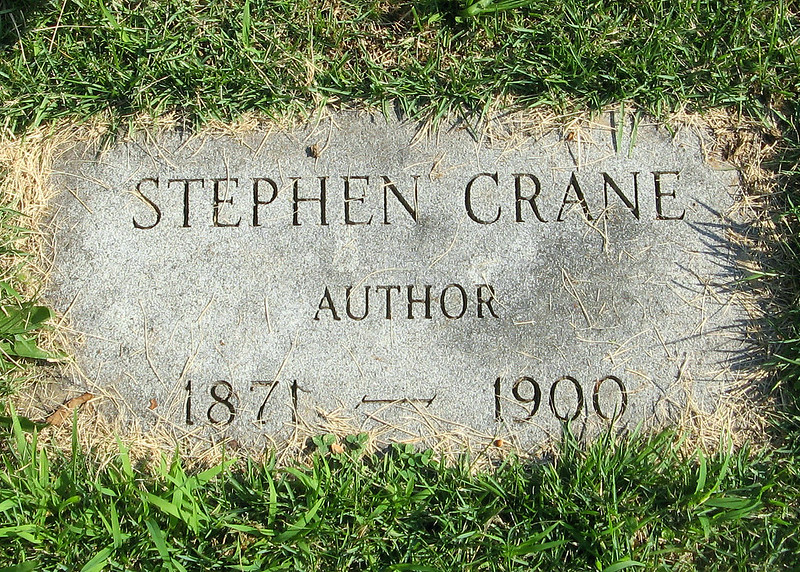
\includegraphics[width=12cm]{Figures/ccby.jpg}
\end{center}
\caption{``\href{https://openverse.org/image/110032f8-1a7a-421f-86b1-88fdfde2e44f
  }{Stephen Crane, Author, Red Badge of Courage}''
  by~\href{https://www.flickr.com/photos/tonythemisfit/}{Tony Fischer
  Photography} is licensed under
\href{https://creativecommons.org/licenses/by/2.0/}{CC BY 2.0}.}
\label{fig:ccbypic}
\end{figure}

The permission can also be from the publisher. For instance, IEEE and
many other publishers have an automated system for granting permission
for theses. Mark the permission in the caption as requested by the
right holder, e.g., “\textcopyright 2022 IEEE. Reprinted, with
permission, from [x].''

Not all figures exceed the threshold of originality. These include,
for example, scientific diagrams and flowcharts. Good research
practices require that even in this case, the source is cited in the
caption (\enquote{Figure from [x].}). However, it would be best to ask
for permission or at least redraw the image. Images with a CC license
are free to use, so long as the terms of use are
followed~\cite{about_cc_licenses}. Even then, the caption must mention
the source (article, website, etc.) and that the image is CC-licensed.

Based on the right to quote, it is possible to take a photocopy,
screenshot or photograph of a work (not the original file) and publish
it, citing the original source in the caption. A critical aspect of
the right to quote is that the use of the image is relevant to the
work, i.e., the image must be related to the subject, and it must be
explained in the text (this applies to all images). Similarly, the
source must be cited in text citations.

Sometimes you may want to use someone else's original image idea as a
basis for your own work. Permission is not required provided that your
work clearly an amply edited version of the original. However, in
accordance with good research practices the type of modification and
source (``Modified/Adapted/Redrawn/Based on/Created using data from
[x]'') and must be declared in the caption. Should you only make minor
edits to the original, separate permission is required. The University
of Oulu Acta Oulu publishing guide~\cite{ronkainen_copyright} has more
details on this topic, and also the proper wordings in
Finnish~\cite{ronkainen_tekijanoikeus}.

When searching for images through an internet image search, it is not
always easy to find the rights holder from whom to request permission
for use. Hunting for a permit can be a demanding task. The easiest way
is to use images and figures from scientific articles (or with open
licenses) as in these the rights holders are clearly declared.

\section{Accessibility}
\label{accessibility}
Put effort into the accessibility of your thesis. The
structure of an accessible document is clear, and the wording is as
understandable as possible. Figures and tables should be given an
alternative text that summarises the information they contain for the
reader. Alternative text is especially important in situations where
the reader cannot see the figure or table, for example due to vision
impairment.  More information on accessible Word documents and
archivable PDF files can be found in the texts of the University of
Oulu Campus ICT~\cite{ictaccessibleword,ictwordpdfa}. You can also
read about the accessibility of mathematical equations in the Campus
ICT text~\cite{ictaccessiblemath}.
